%\documentclass{article}
%\usepackage{pgfplots}
%\usetikzlibrary{math}
%\begin{document}



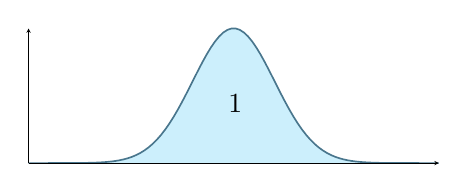
\begin{tikzpicture}[scale=0.5]

\pgfmathdeclarefunction{gauss}{2}{%
  \pgfmathparse{1/(#2*sqrt(2*pi))*exp(-((x-#1)^2)/(2*#2^2))}%
}

\tikzmath{
			\conf = 0; \crit= 1.05; \a=round(1-\conf)/2,2);
          }

%\begin{axis}[
%  no markers, domain=0:10, samples=100,
%  axis lines*=left, xlabel=$x$, ylabel=$y$,
%  every axis y label/.style={at=(current axis.above origin),anchor=south},
%  every axis x label/.style={at=(current axis.right of origin),anchor=west},
%  height=5cm, width=12cm,
%  xtick={4,6.5}, ytick=\empty,
%  enlargelimits=false, clip=false, axis on top,
%  grid = major
%  ]
%  \addplot [fill=cyan!20, draw=none, domain=0:5.96] {gauss(6.5,1)} \closedcycle;
%  \addplot [very thick,cyan!50!black] {gauss(4,1)};
%  \addplot [very thick,cyan!50!black] {gauss(6.5,1)};
%
%
%%\draw [yshift=-0.6cm, latex-latex](axis cs:4,0) -- node [fill=white] {$1.96\sigma$} (axis cs:5.96,0);
%\end{axis}

\begin{axis}[
  no markers, domain=-5:5, samples=100,
  axis lines=left, 
  %xlabel=$xa$, ylabel=$ya$,
  %every axis y label/.style={at=(current axis.above origin),anchor=south},
  %every axis x label/.style={at=(current axis.right of origin),anchor=west},
  height=5cm, width=12cm,
  xtick={\crit}, ytick=\empty,
  xticklabels = { $k$},
  enlargelimits=false, clip=false, axis on top,
  %grid = major
  ]
  \addplot [fill=cyan!20, draw=none, domain=-5:5] {gauss(0,1)} \closedcycle;
  \addplot [very thick,cyan!50!black] {gauss(0,1)};
  %\addplot [very thick,cyan!50!black] {gauss(6.5,1)};
  


%\draw [yshift=-0.6cm, latex-latex](axis cs:4,0) -- node [fill=white] {$1.96\sigma$} (axis cs:5.96,0);
\end{axis}
\node[] at (5.25,1.5) {$1$};	




\end{tikzpicture}

%\end{document}